

\section{The poisson program}
In the beginning I tried to take advantage of our professors framework of several poisson solvers, which uses vectors and matrices in Fortran format. This however turned out to be hard for me. When I tried to create a transpose operation in parallel I could not make it work. So I made a switched to the code distributed with the problemtext, which is written by Einar M. Rønquist. 

\section{Parallelization}
To parallelize the problem I chose to split up the problem in lesser parts, each solvable by it self. Each process generates it own matrix B, and modifies it through the program, before it shares it result with each of the other processes and the maximal error is calculated. During each process' execution the only communication, except for in assembly, between the threads are done in the transpose operation.

\subsection{The transpose operation}
Since each process has a part of the matrix b, a transpose will need to swap elements with other processes. This communcation is done through MPI\_Alltoallv (see figure \ref{fig:transpose}), a MPI call which sends a sendarray according to a count array and a displacement array. The countarray contains the number of elements to be sent to each process. The displacement arrays entry i specifies the displacement relative to the sendarray, entry i is sent to process i. The receive buffer is filled according to the same displacement and count array. 

During the writing of this report, and after results had been obtained, I found that I had created a duplicate matrixAsVec operation. In the transpose operation I believe a less effective version of this has been used, a version not using memcpy(). This may have some small effect on runtime, but no real testing has been performed to confirm this.

% Here insert the illustration of alltoallv from problem text.
\begin{figure}[htbp]
	\centering
	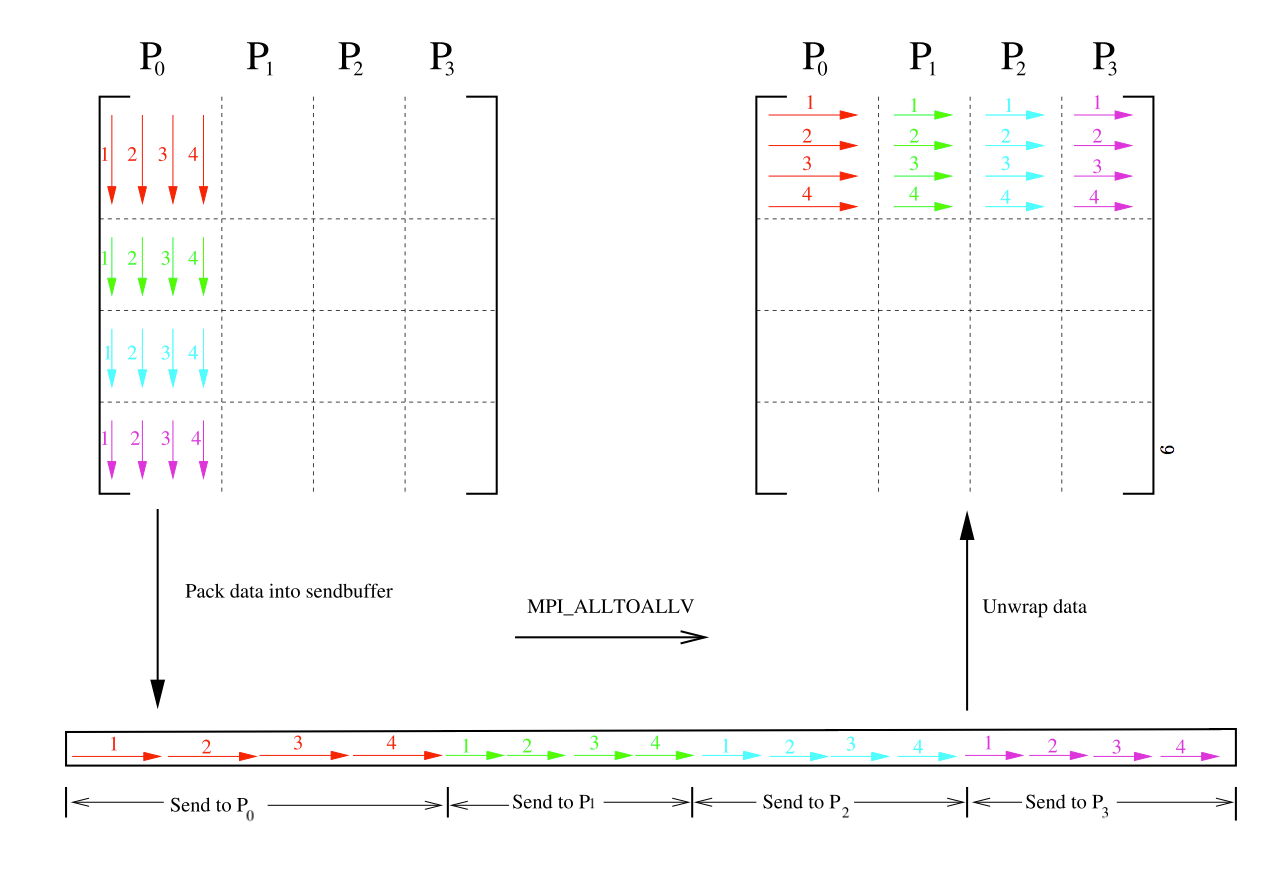
\includegraphics[width=0.8\textwidth]{transpose}
	\caption{Transpose operation through MPI\_Alltoallv}
	\label{fig:transpose}
\end{figure}

\subsection{The error computation in parallel and and results}
At computation of error there is also some need for paralellization. Generation of the problem's exact solution is done for each process', and the exact solution can therefore be compared with the solution found on each process. I here took advantage of our professor's common files, and blaslapack. 

I created a matrixToVec() operation, which transforms the processes part matrix b to a vector, as well as the process' exact solution. After this, an axpy operation is performed on the solution v.s. the exact solution. This performs the following vector operation $y <- (-1.0*solutionVector) + exactVector$. This generates the relative errors for this process' solution. 

Then the maximal local error is found with blas routine idamax, which returns the element of largest magnitude. Now each process has found the max error in it's own part solution. The global max error is computed with a call of MPI\_Reduce with MPI\_MAX, which result in the maximal pointwise error.

For a time I also assembled the final solution matrix on the root process using MPI\_Gatherv. I however found that this was unnecessary, when the results from the program is available in each process, and only the pointwise error is needed for report. 

\subsection{Use of OpenMP}
To further increase the parallelization of the program OpenMP can be used. This enables the program's MPI processes to use more than one thread in it's execution. 
The main (perhaps only) use of extra threads in this program is when performing the fourier transformations. This means adding a 
\begin{lstlisting}
#pragma omp parallel for schedule(static)
\end{lstlisting}
before the various Fortran fourier transformations. This means that each MPI process can perform the fourier transforms with increased degree of parallelization. One drawback with use of OpenMP on these parts of the program is that the fortran procedures requires a buffer. This leads to the requirement of each thread having it's own buffer. This means an increase in memory requirement for the program, due to an increased size of buffer matrix z.

Possible speedup with use of OpenMP will be discussed in result section(INCLUDE REFERENCE TO IT). 



\section{Kongull}
Kongull has 108 compute nodes, each having 2 processors. This is divided in 96 nodes using an AMD Opteron processor with 6 cores, and 12 nodes using Intel(R) Xeon(R) processors. Depending on which rack of the compute nodes are being used, the node has 24 GiB/node or 48 GiB/node. This means that each processor has at least 12 GiB of memory (create reference to https://www.hpc.ntnu.no/display/hpc/Kongull+Hardware Compute-nodes). I believe that our student projects in TMA4280 only have access to the section having 24 GB memory per node. 

To compile and run the program I have used Intel's compilers for Fortran and C, ifortran and icc. Cmake was used to perform the compilation with these compilers. This generates a build system with portability and simplicity. 
The program uses MPI, OpenMP and BLAS/Lapack. In addition support for C99 has been added for simplicty of writing code.
All of these are installed on Kongull.


\section{Verification of correctness}
To verify that the code works correctly, I have performed a convergence test. To obtain a correct error estimate an exact solution were computed. The exact solution has been entered as 
\begin{equation}
	u(x,y) = sin(\pi x) \cdot sin(2\pi x)
\end{equation}
Which satisfies the homogeneous boundary conditions $u = 0 \text{ on } \partial\Omega$. If we then evalueate $-\nabla^2 u$ which should be equal to 
\begin{equation}
	u(x,y) = 5\pi^2 \cdot sin(\pi x) \cdot sin(2\pi x)
\end{equation}
The error gained from comparison of the exact and computed solution is then used to check whether the program performs correctly.

This test has been performed with 3 nodes with 2 processors each having 6 cores. Assigned number of threads per MPI process was 6, which perhaps is not ideal, but nevertheless. The program was executed with this setup for a number of problem sizes from $n=4 8 16 ...16384$, and the errors for each problem size is compared with $h=(1 / n)^2$. This then was processed in a octave plot using loglog, resulting in the following plot \ref{fig:loglogerror} where the gradient $a = 2.0309$ is just about two. The graph is also just about completely linear. This verifies the correctness of the solution. 
\begin{figure}[htbp]
	\centering
	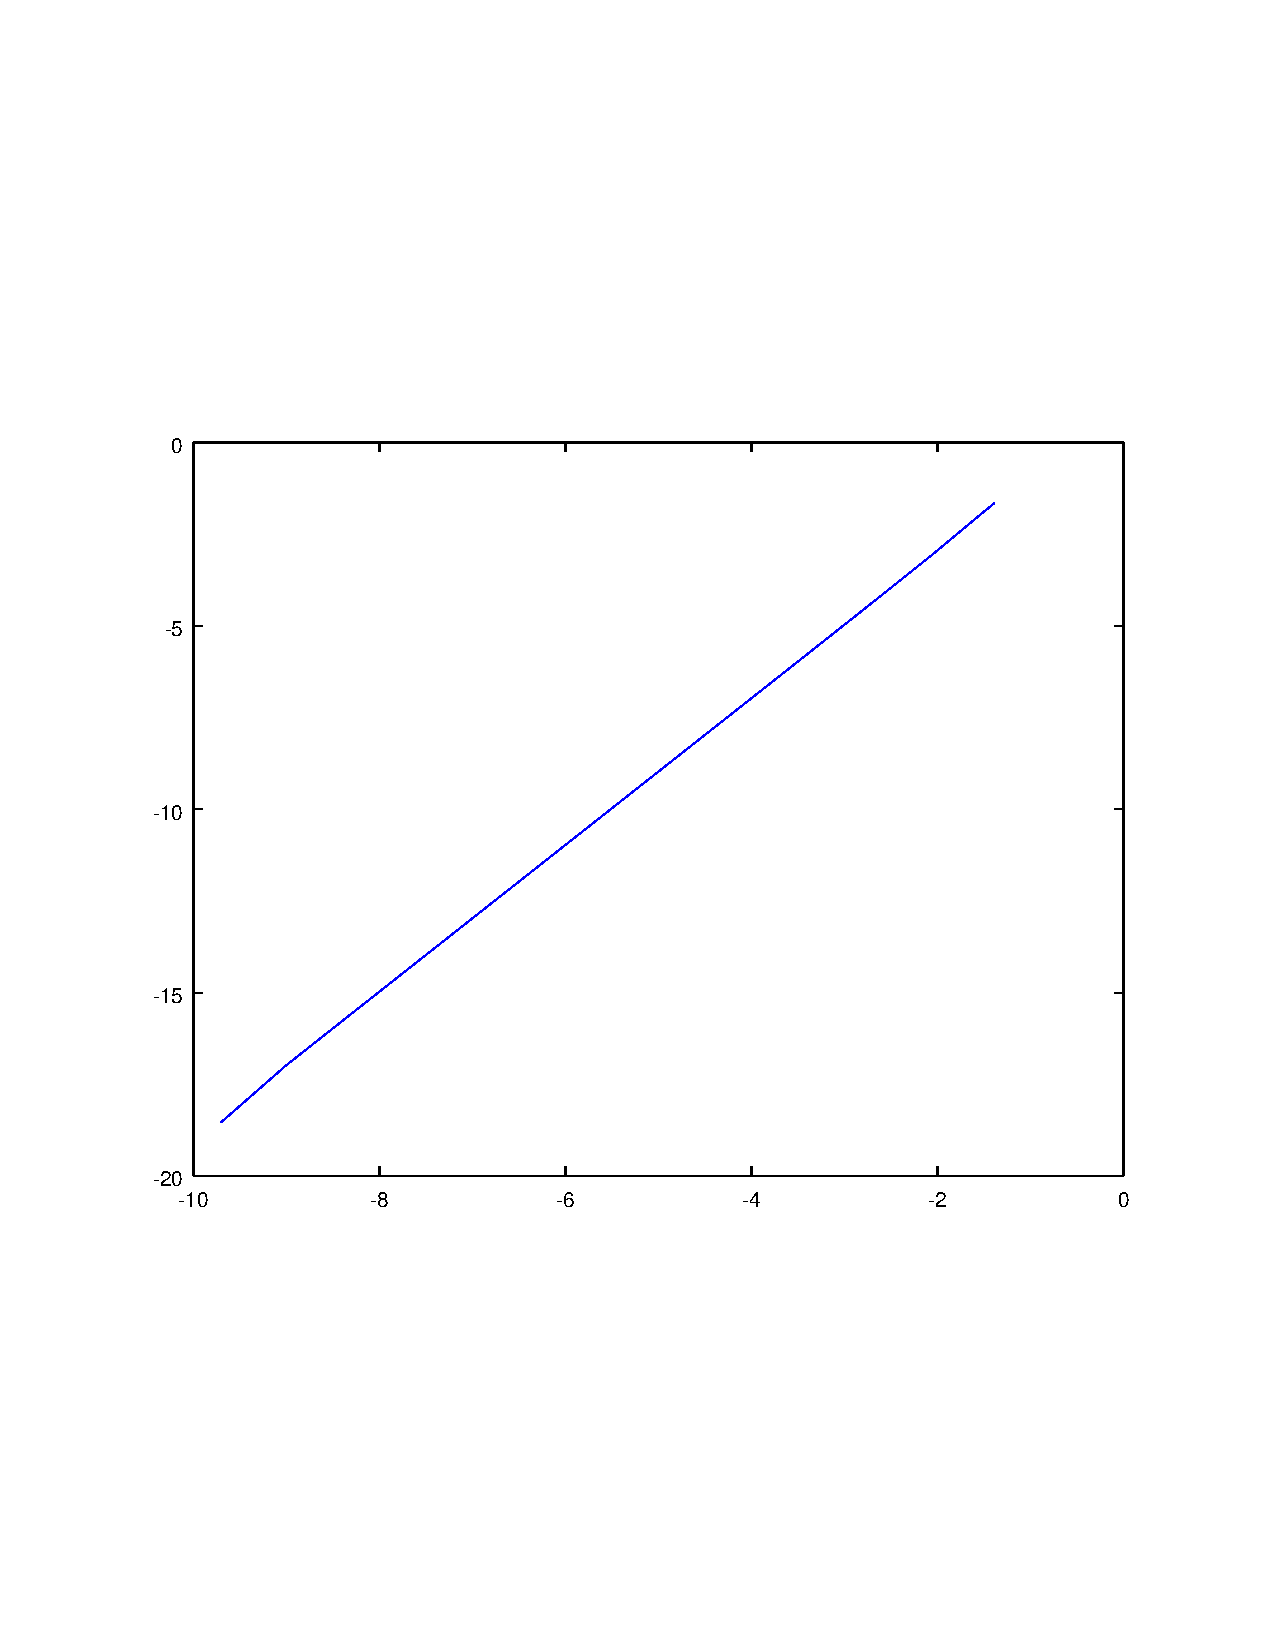
\includegraphics[width=0.8\textwidth]{loglog_error_verification}
	\caption{loglog plot of h, max pointwise error}
	\label{fig:loglogerror}
\end{figure}

\section{Hybrid v.s. Pure distributed memory model}

